\documentclass[tikz,border=3mm]{standalone}
\usetikzlibrary{positioning}

\begin{document}
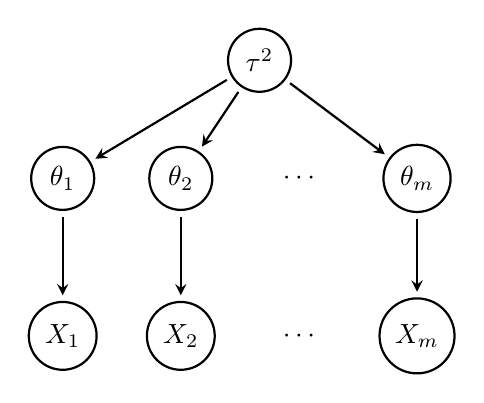
\begin{tikzpicture}[
    node distance=1.5cm and 1.2cm,
    vertex/.style={circle, draw, minimum size=0.8cm, thick},
    arrow/.style={->, thick, >=stealth, shorten >=2pt, shorten <=2pt}
]

% Top level: tau^2
\node[vertex] (tau) at (0,-0.5) {$\tau^2$};

% Middle level: theta_1, ..., theta_m
\node[vertex] (theta1) at (-2.5,-2) {$\theta_1$};
\node[vertex] (theta2) at (-1,-2) {$\theta_2$};
\node (dots1) at (0.5,-2) {$\cdots$};
\node[vertex] (thetam) at (2,-2) {$\theta_m$};

% Bottom level: X_1, ..., X_m
\node[vertex] (x1) at (-2.5,-4) {$X_1$};
\node[vertex] (x2) at (-1,-4) {$X_2$};
\node (dots2) at (0.5,-4) {$\cdots$};
\node[vertex] (xm) at (2,-4) {$X_m$};

% Arrows from tau^2 to all theta_i
\draw[arrow] (tau) -- (theta1);
\draw[arrow] (tau) -- (theta2);
\draw[arrow] (tau) -- (thetam);

% Arrows from each theta_i to corresponding X_i
\draw[arrow] (theta1) -- (x1);
\draw[arrow] (theta2) -- (x2);
\draw[arrow] (thetam) -- (xm);

\end{tikzpicture}
\end{document}